{\documentclass[runningheads]{llncs}
\usepackage{graphicx}
\usepackage{hyperref}
\usepackage{float}
\usepackage{caption}
\usepackage{subcaption}


\begin{document}

\title{Flu Shot Learning: Predict H1N1 and Seasonal Flu Vaccines}

\author{\textbf{MaLuCS Team}\newline Luca Corbucci 516450 \and Cinzia Lestini 219809 \and Marco Giuseppe Marino 596673 \and Simone Rossi 507267}
\institute{University of Pisa
    \\Big Data Analytics
    \\ Academic Year 2020/21}
\maketitle

\begin{abstract}
    During spring 2009 a pandemic caused by the H1N1 influenza virus swept across the world.
    In late 2009 the United States conducted the National 2009 H1N1 Flu Survey \cite{Dataset}.
    Using part of the data collected during this survey we want to predict whether people got H1N1 and seasonal flu vaccines.
    The goal of this report is to explain the most interesting aspects discovered during our project.
    \keywords{Data analysis \and Data visualization \and Flu shot Learning}
\end{abstract}




\section{Introduction}
\subsection{Our problem}

During spring 2009 a pandemic caused by the H1N1 influenza virus swept across the world. Researchers estimate that in the first year, it was responsible for between 151,000 to 575,000 deaths globally.

The first vaccine for this virus became available in October 2009, after some months the United States conducted the National 2009 H1N1 Flu Survey.

In 2020, in the middle of the Covid-19 pandemic, Driven Data proposed a competition \cite{Driven Data} to study the data collected during the 2009 survey.

To let people compete in this challenge Driven Data has made available a Dataset with the results of this survey. The goal is to develop a Machine Learning Model that can predict whether people got H1N1 and seasonal flu vaccines.

\subsection{Dataset Description}

The training dataset provided by Driven Data contains 26707 rows and 38 features. For each row we have an ID that is unique for each respondent, the ID number goes from 0 to 26706.
The features cover various topics from the behavior of the respondents to the economic situation.
For all the columns we did not find any outlier and “strange” value, for this reason, we guess that the respondents had only a fixed number of possible answers for each question or that Driven Data cleaned a bit the dataset before publishing it.

There are two class labels, one for the H1N1 vaccine (“$H1N1\_vaccine$”) and one for the seasonal vaccine (“$seasonal\_vaccine$”).
Both values of the class label are made up of 0 and 1, where 0 is equivalent to not having been vaccinated and 1 to having been vaccinated.
As you can see from the plot \ref{img:balancedtarget}, the $H1N1\_vaccine$ vaccine target is not balanced because we have 21033 respondents who did not receive the vaccine and only 5674 that received the vaccine.
On the contrary, the $seasonal\_vaccine$ target variable is almost balanced because 14272 respondents did not receive the vaccine and 12435 received the vaccine.

\begin{figure}
    \centering
    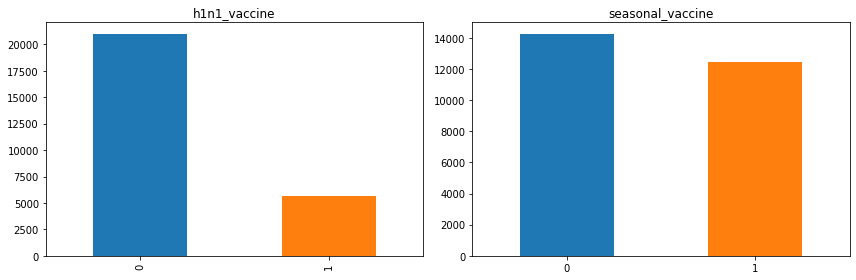
\includegraphics[width=0.7\linewidth]{images/balancedtarget.png}
    \caption{Target distribution}
    \label{img:balancedtarget}
\end{figure}


\section{Data Exploration}

\subsection{Missing Values}

During the data analysis, we noticed that 30 features have at least one missing value.
In most of the cases, we found a low number of missing values concerning the size of our dataset but for 3 attributes we noticed that the missing values were almost half of the total.
We adopted the following approach to deal with missing values:
\begin{itemize}
    \item We deleted the 3 features with half the missing values (\textit{health\_insurance, employment\_industry and employment\_occupation}).
    \item We used the mode to fill most of the other missing values.
          With the most correlated attributes, we grouped the rows using the correlated feature to assign the most likely value to the missing value.
\end{itemize}

\subsection{Features}

In this subsection we briefly describe the types of features of our dataset:

\begin{itemize}
    \item \textbf{Binary features} where the value 0 is equivalent to a negative response and the value 1 to a positive response:
          \begin{itemize}
              \item Seven features, associated with the respondent's preventive behaviour towards flu diseases:“$behavioral\_antiviral\_meds$”,        “$behavioral\_avoidance$”, “$behavioral\_face\_mask$”, “$behavioral\_wash\_hands$”, “$behavioral\_large\_gatherings$”, “$behavioral\_outside\_home$”,“$behavioral\_touch\_face$”.
              \item Two features for the doctor recommendation of the H1N1 and seasonal flu vaccine (“$doctor\_recc\_h1n1$”, “$doctor\_recc\_seasonal$”).
              \item Three feature to understand if the respondent is at higher risk of catching the flu: “$chronic\_med\_condition$”, “$child\_under\_6\_month$”, “$health\_worker$”.
              \item “$Health\_insurance$”.
          \end{itemize}
    \item \textbf{Ordinal categorical} features for different topics, the respondent chooses based on a scale with graded answers:
          \begin{itemize}
              \item Level of concern and knowledge about the H1N1 flu ( “$H1N1\_concern$“, “$H1N1\_knowledge:$”).
              \item Six Features about respondent's opinions about H1N1 and seasonal vaccine effectiveness, getting sick with flu without them and from taking them ($opinion\_h1n1\_vacc\_effective$, $opinion\_h1n1\_risk$, $opinion\_h1n1\_sick\_from\_vacc$, $opinion\_seas\_vacc\_effective$, etc..).
          \end{itemize}
    \item \textbf{Nominal categorical} features concerning the personal data of the respondent:
          \begin{itemize}
              \item “$age\_group$”, “education level”, “race”, “sex”, “marital status”, “$rent\_or\_own$”, “marital status”,“employment status”, “$census\_msa$” that is the respondent's residence as defined by the U.S. Census.
              \item Three features about the respondent's residence and occupation, the values are encoded in random strings to preserve privacy (“$hhs\_geo\_region$”, “$employment\_industry$”, ”$employment\_occupation$”).
          \end{itemize}
    \item Numeric features concerning the size of the family “$household\_adults$, “$household\_children$”.
\end{itemize}

In Figure \ref{img:hist} we show some examples of the bar charts of different features.

\begin{figure}
    \centering
    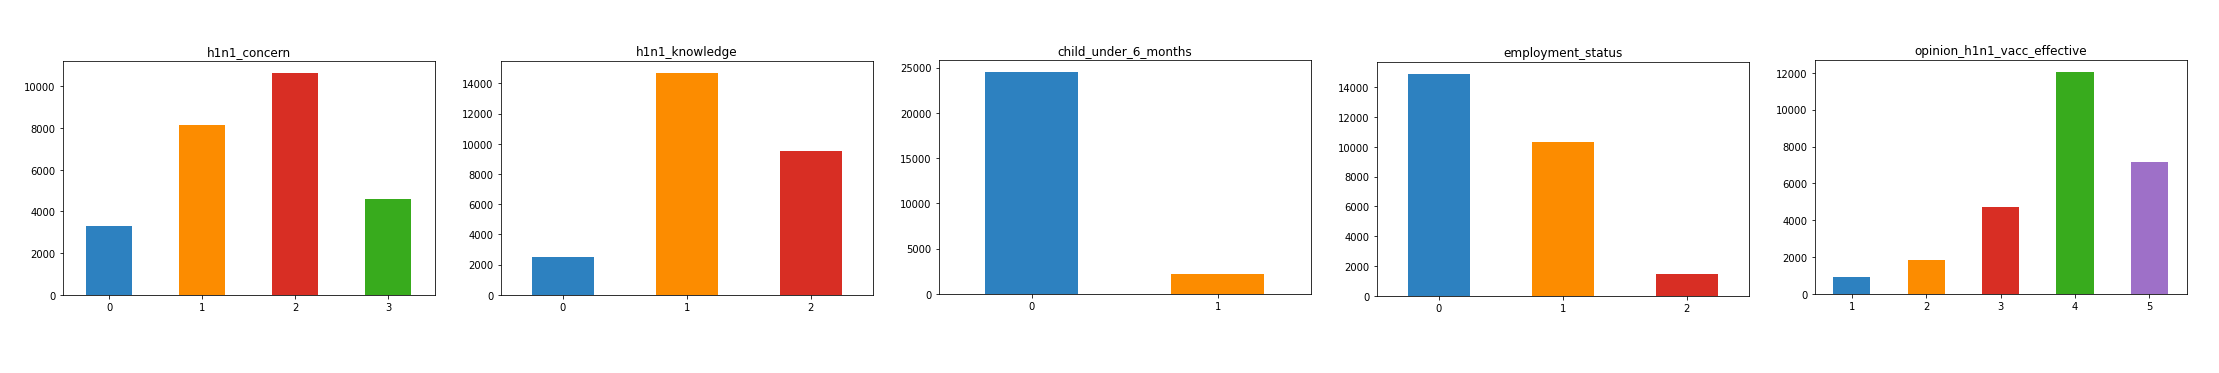
\includegraphics[width=\linewidth]{images/uniti.png}
    \caption{Distribution of some of our variables}
    \label{img:hist}
\end{figure}

\subsection{Conditional Bar chart}

An important part of the data exploration was the study of the variables conditional distributions.
We aimed to understand how a certain feature can discriminate the target variables. We noticed that there exist some features where an answer strongly implies a certain target variable while there exist other variables that are not too much discriminant.

Here we report only the most interesting plots, the full set of the plots is available in our notebook.

In Figure \ref{img:levelofconcern} we can see that a respondent with high concern about the H1N1 flu will be more likely to receive not only the H1N1 vaccine but also the seasonal vaccine.

We have a similar situation also with the feature “$opinion\_h1n1\_vacc\_effective$” and with “$opinion\_h1n1\_risk$”, in this case, we have that a respondent that thinks that the H1N1 vaccine will be effective or that have fear of the H1N1 flu will be more likely to also receive the seasonal vaccine.

As we expected, the presence of the chronic medical condition is important information to consider, especially for the seasonal vaccine.
You can see in \ref{img:chronic} that almost $60\%$ of the respondents with chronic medical conditions received the seasonal vaccine.

\begin{figure}
    \begin{minipage}{0.48\textwidth}
        \centering
        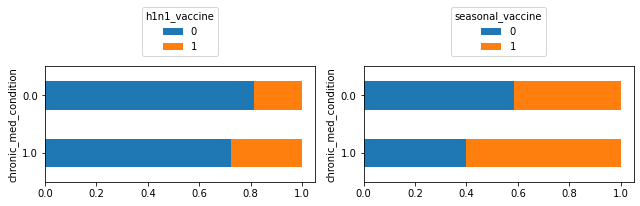
\includegraphics[width=\linewidth]{images/chronic_med.png}
        \caption{The respondent have at least one of a set of chronic medical conditions}\label{img:chronic}
    \end{minipage}\hfill
    \begin{minipage}{0.48\textwidth}
        \centering
        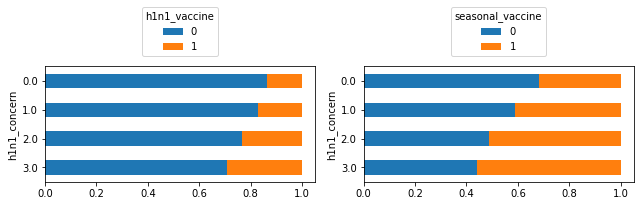
\includegraphics[width=\linewidth]{images/h1n1_concern.png}
        \caption{Level of concern about the H1N1 flu. 0 is Not at all concerned, 3 is Very concerned}\label{img:levelofconcern}
    \end{minipage}
\end{figure}



The feature “$age\_group$” gives us rather obvious information\ref{img:age_group}, the older the age of the respondents the more likely they are to receive the vaccine. However, this assumption is valid only for the seasonal vaccine while for the H1N1 vaccine we did not find a strong correlation with this information.

\begin{figure}
    \centering
    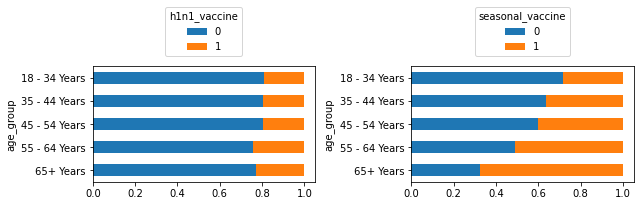
\includegraphics[width=0.8\linewidth]{images/age_group.png}
    \caption{Age group of respondent.}
    \label{img:age_group}
\end{figure}

\subsection{Correlation}
\label{sec:correlation}

The last aspect of our dataset we need to explore is the correlation between features. This study is important because it helps us in the data transformation phase. Indeed, correlation gives us the information needed to decide if we have to keep, discard, or transform a feature.
We used the Pearson linear correlation coefficient to correlate our columns.

In figure \ref{heatmap_correlation} we show the heatmap for the correlation analysis we computed, the feature “$H1N1\_concern$” shows overall a weak correlation with the features about behavior and opinion becoming a candidate for elimination.
Except for “$behavioral\_antiviral\_meds$” and “$behavioral\_face\_mask$” features, all the “$behavioral$” attributes show between each other some kind of correlation.


\begin{figure}
    \centering
    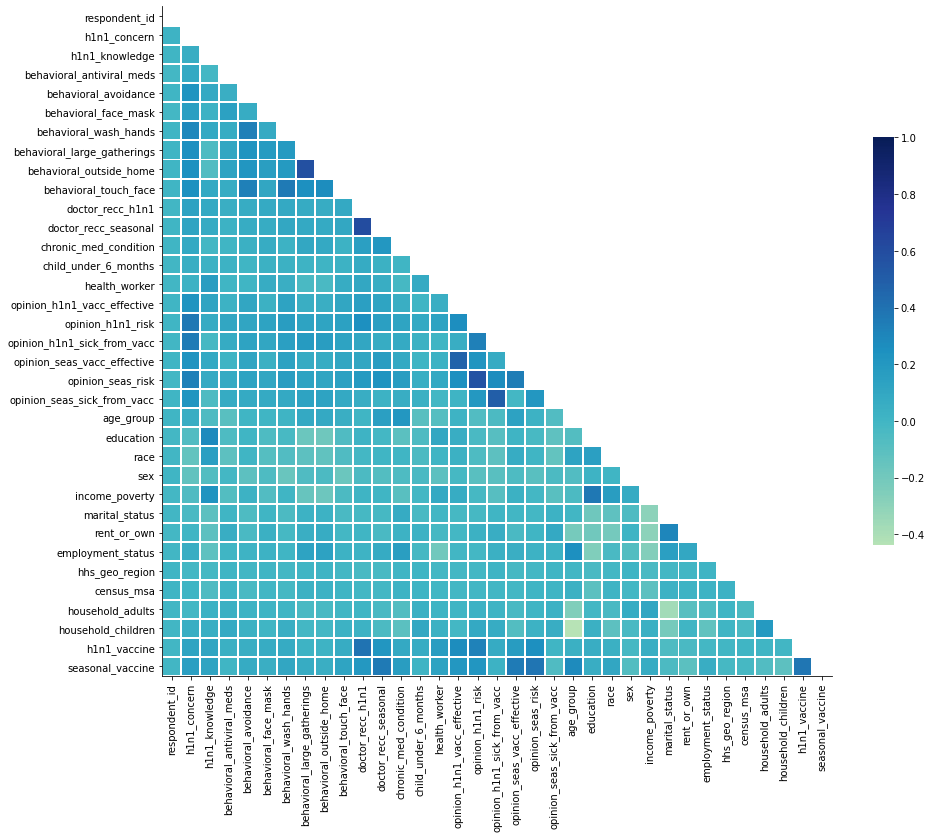
\includegraphics[width=0.5\linewidth]{./images/heatmap.png}
    \caption{Correlation of our features}
    \label{heatmap_correlation}
\end{figure}


This may let us create a new feature starting from them that makes our dataset simpler and more understandable. “$opinion\_h1n1\_vacc\_effective$” is weakly related to “$opinion\_h1n1\_risk$” and this last feature has a moderate correlation with “$opinion\_h1n1\_sick\_from_vacc$”.
“$opinion\_h1n1\_vacc\_effective$” and “$opinion\_h1n1\_sick\_from\_vacc$” have no significant correlation.
The same behavior is followed by the “opinion” attributes regarding the seasonal flu vaccine and the pairs of “opinion” of the two vaccines are respectively correlated.
We can also emphasize the correlation between the features regarding the social-economic background of the recipient.
At this point, we studied the correlation of the attributes with the target features to get a better idea of their importance. For “$H1N1\_vaccine$” we can emphasize the correlation with : “$doctor\_recc\_h1n1$”, “$opinion\_h1n1\_risk$” and “$opinion\_h1n1\_vacc\_effective$”.
For “$seasonal\_vaccine$” we have: “$opinion\_seas\_risk$”, “$doctor\_recc\_seasonal$”, “$opinion\_seas\_vacc\_effective$” and “$age\_group$”.
We can conclude that in general, we have not observed very strong correlations in our dataset.

\section{Data Transformation}

In this section, we proceed towards the manipulation and transformation of our dataset as a consequence of the results we previously collected and analyzed.

\subsection{Variables Elimination}

We dropped from our dataset all the features we believed are not fundamental for the classification task. In particular, we can safely delete variables that are correlated with others that remain in the dataset.
In particular, we removed: “$H1N1\_concern$”, “$rent\_or\_own$”, “$behavioral\_large\_gatherings$”, “$marital\_status$” and “education”. Some variables that may be useless for the classification task, cannot be deleted a priori because they are not correlated with other non-target features.

\subsection{Creating new variables}
We have created two new attributes: 'FamilySize', which tells us the size of the family of the respondent including the respondent, and 'Behaviour', which represents the sum of the values of the behavioral attributes.
We noticed that merging the behavioral features into a single attribute does not create substantial differences because, as we said in Section \ref{sec:correlation}, these features are correlated.
The individual attributes used to create the new attributes have been removed from the dataset.



\section{Balancing the dataset}
\label{sec:balancing}

The H1N1 vaccine dataset is numerous, it contains 26707 rows, but it is not balanced because we have 79\% respondents who did not receive the vaccine (class 0) and only 21\% received the vaccine (class 1).
This imbalance has negative effects on the performance of class 1, on the applied training models.
We balanced both the full and reduced H1N1 vaccine dataset with new variables.
We chose the decision tree classifier as the comparison model and searched for the best hyperparameters for each dataset.
To balance the dataset we have thus used various methodologies:
\begin{itemize}
    \item Under Sampling
    \item Over Sampling
    \item Smote
    \item Adasyn
    \item Under/Over Sampling
    \item Over/Under
    \item Under/Smote
    \item Over/Smote
    \item Class Weight.
\end{itemize}

We have devised a function for each method that looks for the best sampling percentages. The function samples the dataset with all the possible sampling percentages, for each sampling it applies the same Decision Tree Model with selected hyperparameters and gives out the performance values and the summary figures of them.
The winner methodology was chosen, comparing the performance of the same classifier after balancing the dataset with the best sampling percentage of each methodology, we show the comparison in Figure \ref{img:balancing_plot}.

\begin{figure}
    \begin{minipage}{0.32\textwidth}
        \centering
        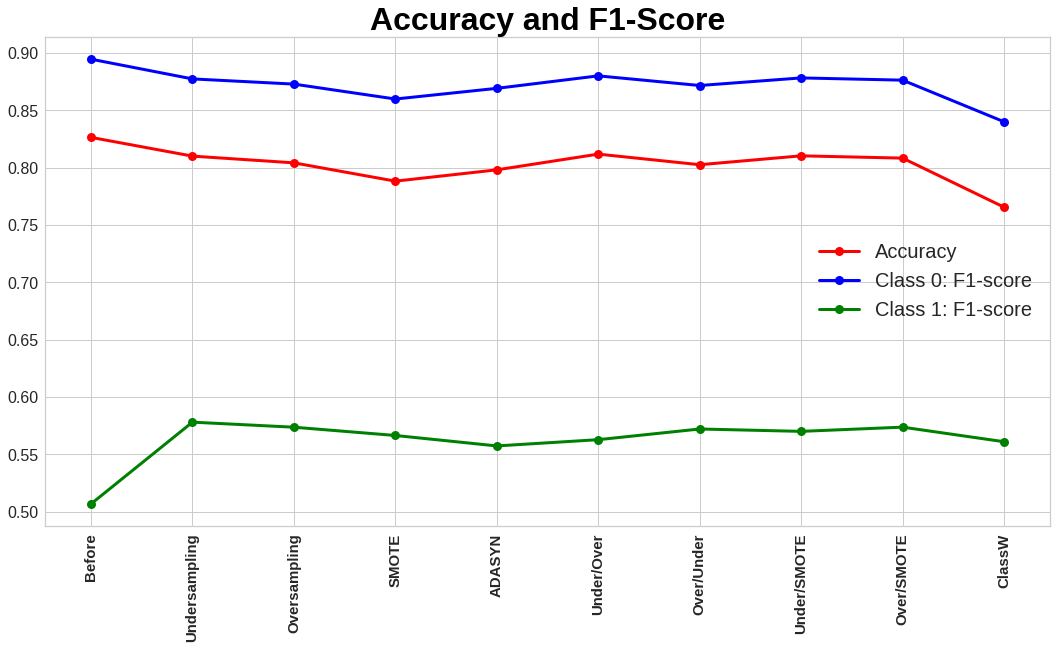
\includegraphics[width=\linewidth]{images/01_balance.png}

    \end{minipage}\hfill
    \begin{minipage}{0.32\textwidth}
        \centering
        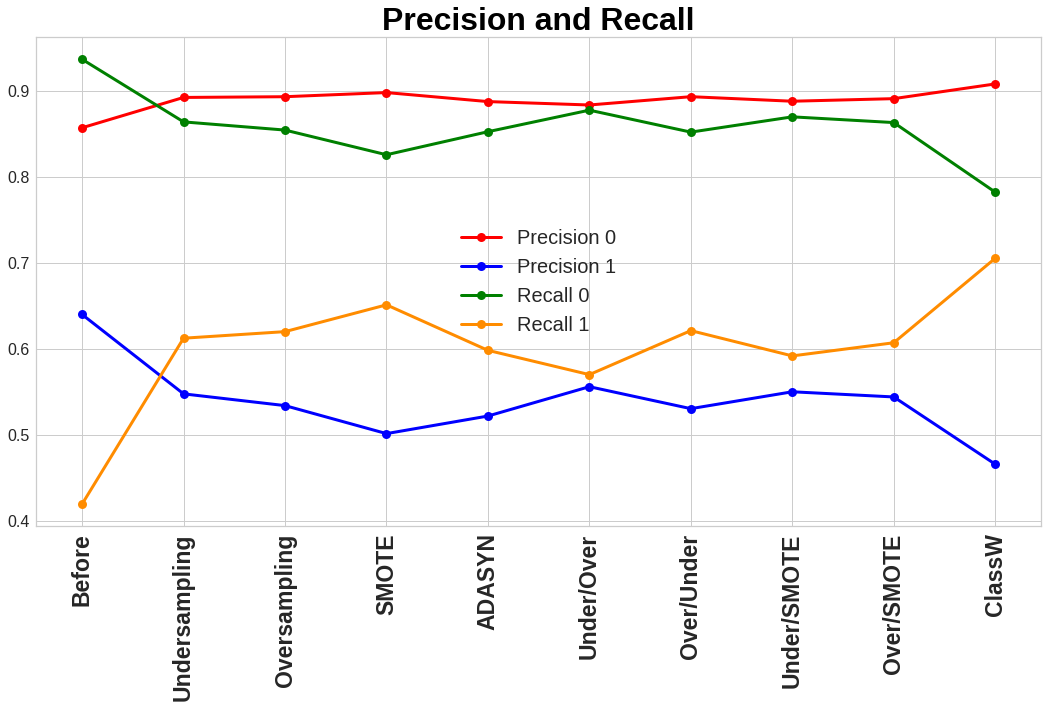
\includegraphics[width=\linewidth]{images/02_balance.png}

    \end{minipage}
    \begin{minipage}{0.32\textwidth}
        \centering
        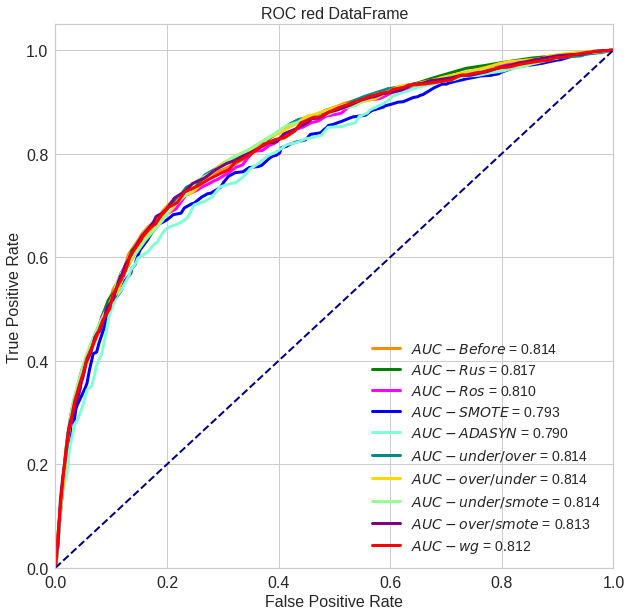
\includegraphics[width=\linewidth]{images/03_balance.png}

    \end{minipage}
    \caption{Comparison of different balancing methods for the H1N1 vaccine dataset}
    \label{img:balancing_plot}
\end{figure}


We noticed that the recall and precision values for each class were symmetrical, that is, as one value increases, the other decreases and vice-versa.
In the end, we decided that choosing the best method is a compromise between a good F1-score of class 1 and a good value of Accuracy and Auc.
For the H1N1 vaccine (reduced dataset), the best method is the Under Sampling with a sampling rate of 0.6, a 0,81 Accuracy, and 0,817 Auc. The latter value remains similar to the pre-sampling while there is an improvement in the F1-score of class 1, which changes from a value of 0.51 to a maximum value of 0.58.
In Figure \ref{img:pca_balancing} we can see the scatter plot of PCA on the reduced H1N1 dataset with the distribution of class labels before and after under-sampling.

\begin{figure}
    \begin{minipage}{0.48\textwidth}
        \centering
        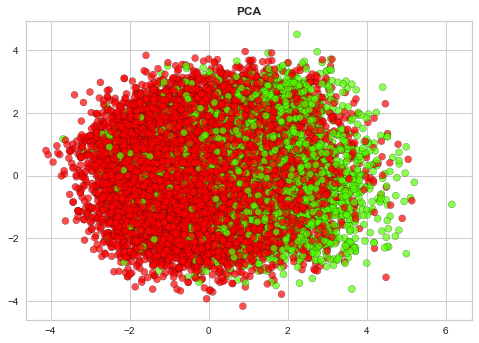
\includegraphics[width=\linewidth]{images/04_balance.png}

    \end{minipage}\hfill
    \begin{minipage}{0.48\textwidth}
        \centering
        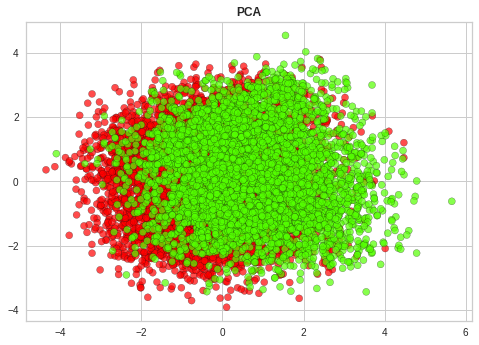
\includegraphics[width=\linewidth]{images/05_balance.png}

    \end{minipage}
    \caption{PCA scatter plot for the H1N1 vaccine before and after Under Sampling}
    \label{img:pca_balancing}
\end{figure}

In the end, we have reached a satisfactory final result but, despite having explored many balancing methods, not as desired because class 1 did not improve significantly.

\section{Data Transformation Assessment}

Before moving to the training of the models we have to check the quality of the decisions we made in the Data Transformation phase. We have to assess at first the splitting of the main dataset into two sub-datasets one for the Seasonal flu and one for the H1N1 and then we need to understand if we have made a good choice in the creation of the “behavior” and “FamilySize” variables.
To solve the first problem we have trained a Decision Tree on the complete dataset and one on the sub-dataset for both targets: “$seasonal\_vaccine$” and “$H1N1\_vaccine$”.
We have to reason in terms of the difference in important features, accuracy, and F1 score.
For the H1N1 we have:

\begin{table}
    \centering
    \begin{tabular}{|c|c|c|c|c|}
        \hline
        H1N1    & Feature Importance         & Accuracy                        & F1 (0)                     & F1 (1)                     \\
        \hline
        Full    & \begin{tabular}{@{}c@{}}$doctor\_recc\_h1n1$, $opinion\_h1n1\_risk$,  \\ $opinion\_h1n1\_vacc\_effective$\end{tabular} & \multicolumn{3}{c|}{Difference}                                                           \\
        \hline
        Reduced & \begin{tabular}{@{}c@{}}$doctor\_recc\_h1n1$, $opinion\_h1n1\_risk$,  \\ $opinion\_h1n1\_vacc\_effective$\end{tabular} & \begin{tabular}{@{}c@{}}Tr:0.004  \\ Ts:-0.007\end{tabular}      & \begin{tabular}{@{}c@{}}Tr:0.002  \\ Tr:0.002\end{tabular} & \begin{tabular}{@{}c@{}}Tr:0.01
            \\ Ts:-0.004\end{tabular} \\
        \hline
    \end{tabular}
    \label{tab:my_label}
    \vspace{-4mm}
\end{table}



For the Seasonal vaccine we have:

\begin{table}
    \centering
    \begin{tabular}{|c|c|c|c|c|}
        \hline
        Seasonal & Feature Importance         & Accuracy                        & F1 (0)                     & F1 (1)                     \\
        \hline
        Full     & \begin{tabular}{@{}c@{}}$opinion\_seas\_vacc\_effective$, $ doctor\_recc\_seasonal, $  \\ $opinion\_seas\_risk $\end{tabular} & \multicolumn{3}{c|}{Difference}                                                           \\
        \hline
        Reduced  & \begin{tabular}{@{}c@{}}$opinion\_seas\_vacc\_effective$, $ doctor\_recc\_seasonal$,  \\ $opinion\_seas\_risk $\end{tabular} & \begin{tabular}{@{}c@{}}Tr:0.003
            \\ Ts:-0.003\end{tabular}      & \begin{tabular}{@{}c@{}}Tr:0.005  \\ Ts:-0.001\end{tabular} & \begin{tabular}{@{}c@{}}Tr:0.0008
            \\ Ts:-0.0068\end{tabular} \\
        \hline
    \end{tabular}
    \label{tab:my_label}
    \vspace{-4mm}
\end{table}

As we can see from those tables we have no relevant differences between the two datasets therefore to improve the explainability and simplicity we decided to use the reduced one.
We used the same process to do our tests on the introduction of the new variables. We have trained a Decision Tree on the dataset with the new features and one on the dataset with the old columns.
For the H1N1 we have:


\begin{table}[H]
    \centering
    \begin{tabular}{|c|c|c|c|c|}
        \hline
        H1N1    & Feature Importance         & Accuracy                        & F1 (0)                     & F1 (1)                     \\
        \hline
        Full    & \begin{tabular}{@{}c@{}}$doctor\_recc\_h1n1$, $ opinion\_h1n1\_risk, $  \\ $opinion\_h1n1\_vacc\_effective$\end{tabular} & \multicolumn{3}{c|}{Difference}                                                           \\
        \hline
        Reduced & \begin{tabular}{@{}c@{}}$doctor\_recc\_h1n1$, $opinion\_h1n1\_risk$,  \\ $opinion\_h1n1\_vacc\_effective$\end{tabular} & \begin{tabular}{@{}c@{}}Tr:-0.001\\ Ts:0.0008\end{tabular}      & \begin{tabular}{@{}c@{}}Tr:0.001  \\ Ts:0.001\end{tabular} & \begin{tabular}{@{}c@{}}Tr:-0.01
            \\ Ts:-0.01\end{tabular} \\
        \hline
    \end{tabular}
    \label{tab:my_label}
    \vspace{-4mm}
\end{table}

For the Seasonal vaccine we have:


\begin{table}[H]
    \centering
    \begin{tabular}{|c|c|c|c|c|}
        \hline
        Seasonal & Feature Importance         & Accuracy                        & F1 (0)                     & F1 (1)                     \\
        \hline
        Full     & \begin{tabular}{@{}c@{}}$opinion\_seas\_vacc\_effective$, $doctor\_recc\_seasonal$,  \\ $opinion\_seas\_risk$\end{tabular} & \multicolumn{3}{c|}{Difference}                                                           \\
        \hline
        Reduced  & \begin{tabular}{@{}c@{}}$opinion\_seas\_vacc\_effective$, $doctor\_recc\_seasonal$,  \\ $opinion\_seas\_risk$\end{tabular} & \begin{tabular}{@{}c@{}}Tr:-0.0028\\ Ts:0.0022\end{tabular}      & \begin{tabular}{@{}c@{}}Tr:-0.005  \\ Ts:-0.0002\end{tabular} & \begin{tabular}{@{}c@{}}Tr:0.0008 \\ Ts:0.005\end{tabular} \\
        \hline
    \end{tabular}
    \label{tab:my_label}
    \vspace{-4mm}
\end{table}

Similar to the first problem we do not have any significant difference so we will use the reduced dataset with the new variables “behavior” and “FamilySize”.

\section{Modeling}

During the classification phase, we tried several different models and in the end, we selected the most interesting ones. In this section, we will explain why we decided to use them.

\begin{itemize}
    \item Decision Tree: they are easy to explain \cite{dtInterpretability} because they can be expressed in a sort of rule language with conditions.
    \item Random Forest: it is an ensemble classifier, we decided to use it to improve the performances of the decision tree.
    \item XGBoost: it is an ensemble classifier, we decided to use it to improve the performances of the decision tree.
    \item SVM: We wanted to make a comparison between Decision Tree and a more complex model
    \item Logistic Regression: it models the probabilities for classification problems with two possible outcomes. We decided to use it because it is interpretable \cite{logisticInterpretability}.
    \item Neural Network: these models are the most complex, we decided to use them because we had a lot of data in our dataset. Unlike Decisions Trees are difficult to interpret.
\end{itemize}

\subsection{Hyperparameters Selection}
\label{sec:hypSelection}
Each of these models has a set of hyperparameters, we used the methods RandomizedSearchCV \cite{RandomizedSearchCV} and GridSearchCV \cite{GridSearchCV} offered by scikit-learn to discover the best ones for our models.

To select the best hyperparameters we followed two different approaches based on the target:
\begin{itemize}
    \item To classify the Seasonal Vaccine we looked for the model with the best accuracy because the two classes were balanced and also because the F1 Score of both classes was always good during our tests.
    \item To classify the H1N1 vaccine we had to deal with an unbalanced dataset and, as we explained in \ref{sec:balancing} we used several techniques. Despite the techniques we applied, we always had a bad F1 score during our tests and so for this dataset, we decided to use the F1 Score as our metric and so we tried to maximize this during the Grid Search.
\end{itemize}

To select the best hyperparameters we have split our dataset into three parts:
\begin{itemize}
    \item Training Set: we used this set of data to train our model.
    \item Validation Set: we used this set to choose the best hyperparameters.
    \item Test set: we used this set to understand the performances of the models.
\end{itemize}

DrivenData also provided us a test set without labels that we can use to make predictions and to upload them to join the competition. We will talk more about this in subsection \ref{sec:testSetResults}.

\section{Model Comparison}

In this section, we want to compare the models that we trained and to reason about what could be the best for our problem.

\subsection{Seasonal}


\begin{table}[!htb]
    \centering
    \begin{tabular}{|c|c|}
        \hline
        Model               & Accuracy \\
        \hline
        Dummy model         & 0.50     \\
        \hline
        Decision Tree       & 0.77     \\
        \hline
        Random Forest       & 0.78     \\
        \hline
        XGBoost             & 0.78     \\
        \hline
        SVM                 & 0.78     \\
        \hline
        Logistic Regression & 0.78     \\
        \hline
        Neural Network      & 0.78     \\
        \hline
    \end{tabular}
    \caption{Seasonal dataset model comparison}
    \label{table:seasonal_testSet}
    \vspace{-10mm}
\end{table}

Concerning the seasonal dataset, considering the Figure \ref{img:seasonal_comparison} we can say that all the models have decent accuracy, the best one is the XGBoost, however, it is not too different with respect to the decision tree and the latter is more interpretable so we can conclude that to classify the seasonal dataset we will use the "Decision Tree" because of the good performances, the simplicity of the model and its interpretability.

\begin{figure}[!htb]
    \begin{minipage}{0.48\textwidth}
        \centering
        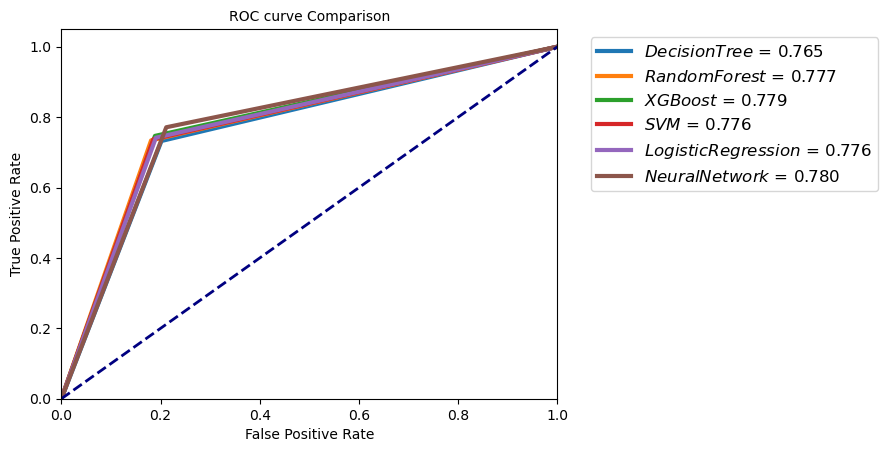
\includegraphics[width=\linewidth]{images/Roc_Curve_seasonal.png}
    \end{minipage}\hfill
    \begin{minipage}{0.48\textwidth}
        \centering
        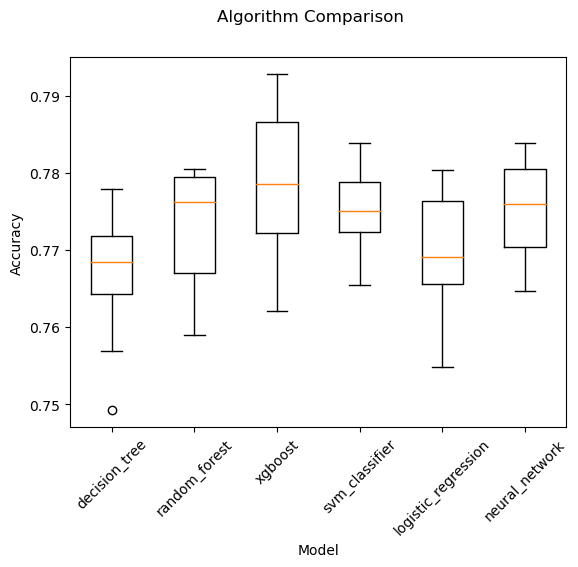
\includegraphics[width=\linewidth]{images/BoxPlot_risultati_Seasonal.png}
    \end{minipage}
    \caption{BoxPlot and Roc curve to compare all the classifiers on the seasonal dataset}
    \label{img:seasonal_comparison}
\end{figure}


\subsection{H1N1}

\begin{table}[H]
    \centering
    \begin{tabular}{|c|c|c|}
        \hline
        Model               & Accuracy & F1-Score \\
        \hline
        Dummy model         & 0.58     & 0.29     \\
        \hline
        Decision Tree       & 0.80     & 0.58     \\
        \hline
        Random Forest       & 0.82     & 0.58     \\
        \hline
        XGBoost             & 0.81     & 0.58     \\
        \hline
        SVM                 & 0.81     & 0.56     \\
        \hline
        Logistic Regression & 0.79     & 0.58     \\
        \hline
        Neural Network      & 0.73     & 0.54     \\
        \hline
    \end{tabular}
    \caption{H1N1 dataset model comparison}
    \label{table:h1n1_testSet}
    \vspace{-10mm}
\end{table}

With the H1N1 dataset, we had more troubles because, as you can see in Table \ref{table:h1n1_testSet} and in Figure \ref{img:h1n1_comparison} the F1-Score for class 1 is always a bit low while the accuracy is decent.
In this case, all the models have similar performances except for the Neural Network, we thought that this is caused by the smaller dataset with respect to the season because of the under-sample.
In the end, also, in this case, we can use the Decision Tree as our best model because it has a good trade-off between performances and interpretability.



\begin{figure}[!htb]
    \begin{minipage}{0.48\textwidth}
        \centering
        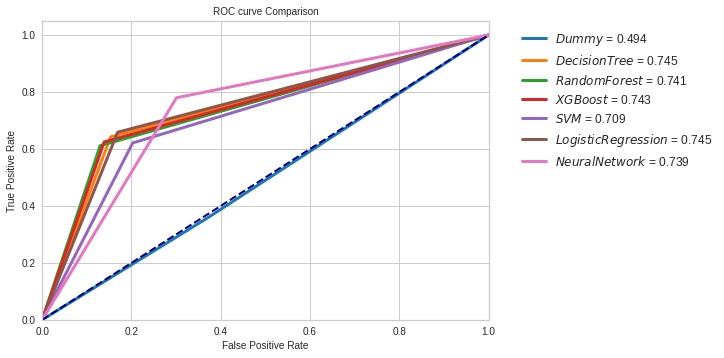
\includegraphics[width=\linewidth]{images/Roc_Curve_h1n1.png}

    \end{minipage}\hfill
    \begin{minipage}{0.48\textwidth}
        \centering
        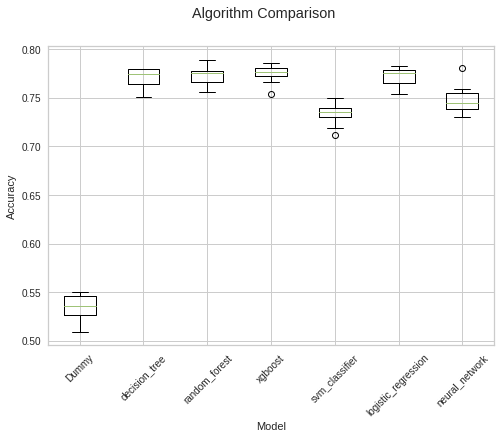
\includegraphics[width=\linewidth]{images/BoxPlot_risultati_h1n1.png}

    \end{minipage}
    \caption{BoxPlot and Roc curve to compare all the classifiers on the H1N1 dataset}
    \label{img:h1n1_comparison}
\end{figure}

\subsection{Test set results}
\label{sec:testSetResults}

As we explained in \ref{sec:hypSelection}, DrivenData provides us an unlabeled test set to take part in the competition.
In the end, we developed a pipeline to clean this test set and to transform it so that it can be used as input in our models.
We used three of our models to make predictions on this test set and we uploaded the results on DrivenData obtaining the following results:

\begin{itemize}
    \item Decision Tree: 0.7424
    \item Random Forest: 0.7469
    \item Neural Network: 0.7499
\end{itemize}

With these scores, we are 373 in the rank with 1455 competitors.

\section{Features Selection}

We decided to apply to our best models a process of feature selection to eventually simplify them further for the stage of interpretation/explanation. We used the RFE of sklearn and the function RFECV from the library yellowbrick.
This last method applies the feature ranking with recursive feature elimination and cross-validation on any not trained classifier of sklearn. It also gives a nice graphical representation of this process that we report in Figure. We identified the best trade-off between the RFECV score and the number of features to use in the models we will interpret and explain. We used the ranking to find out which features we must keep for each model. We keep 8 features for the Seasonal flu XGBoost, 9 columns for the Seasonal flu Decision Tree, 12 features for the h1n1 Random Forest, and 6 columns for the h1n1 Decision Tree.


\begin{figure}
    \begin{minipage}{0.32\textwidth}
        \centering
        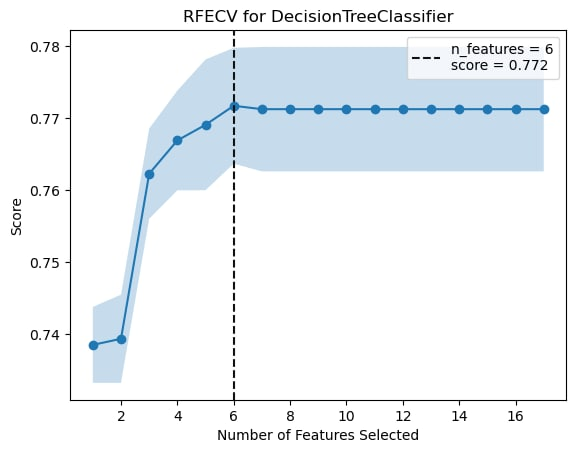
\includegraphics[width=\linewidth]{images/feature_selection1.jpg}

    \end{minipage}\hfill
    \begin{minipage}{0.32\textwidth}
        \centering
        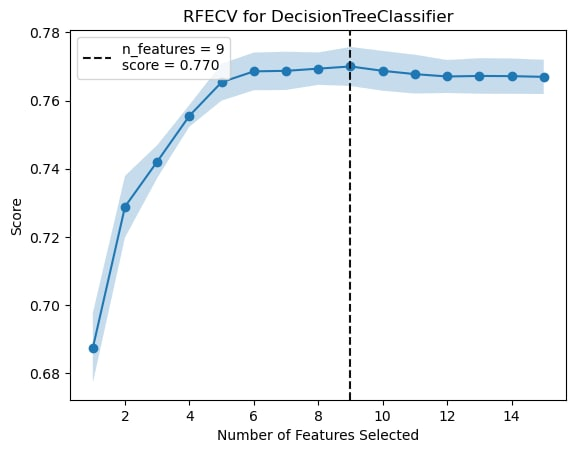
\includegraphics[width=\linewidth]{images/feature_selection2.jpg}

    \end{minipage}
    \begin{minipage}{0.32\textwidth}
        \centering
        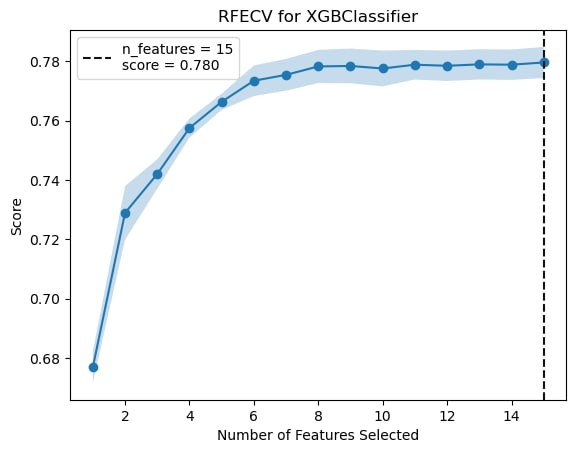
\includegraphics[width=\linewidth]{images/feature_selection3.jpg}

    \end{minipage}
    \caption{Results of the feature selection}
    \label{img:feature_selection}
\end{figure}


\section{Models Explanation}

\subsection{Local Explanation}

The approach we used for the local explanation was the following one:
\begin{itemize}
    \item We selected a set of instances to cover all the possible combinations of predictions and true value so that we could have a better understanding of the model.
    \item Then we used three different local explainers to understand why the model outputs a certain outcome for each record. In particular, we used the following local explainers:
          \begin{itemize}
              \item Lime \cite{molnar2019}
              \item Shap \cite{lundberg2017unified}
              \item Lore \cite{guidotti2018local}
          \end{itemize}
\end{itemize}

\subsection{Comparison of local explanations}

Due to page limits, we report here only one explanation (you can find all the others in the notebook).

\textbf{Local Shap}

The local Shap \cite{lundberg2017unified} plot is called force plot, you can see it in Figure \ref{img:shap_1} it shows how the expected probability of classification for a record is derived, starting from the base value, for the influence of the different features with respect to a certain trained model. In our case, the base value is relative to the probability of classification of the value 1 of the target feature with respect to the relative model. We decided to use the probability scale for simplicity.
Let’s analyse an example from the Seasonal flu XGBoost model:
$y\_pred$ = 0, $y\_true$ = 0, record index  = 5238 and expected probability = 0.05

\begin{figure}[H]
    \centering
    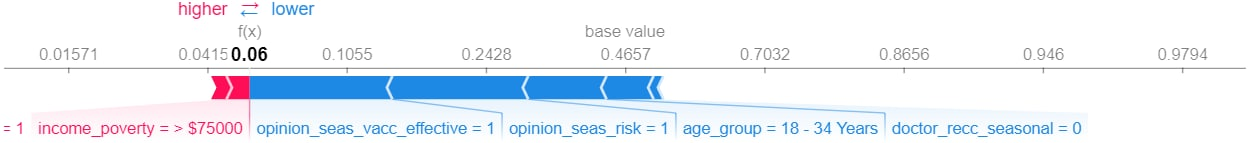
\includegraphics[width=\linewidth]{images/Explanation_Shap_1.png}
    \caption{Shap explanation of a record with true target 0 and predicted target 0}
    \label{img:shap_1}
\end{figure}


This respondent has been correctly classified as 0. Shap tells us that the probability of him being classified as 1 is near 0 because he believes that the vaccine is not effective,  he is young, he is not at risk of taking the flu and the doctor does not recommend the vaccine.

All the records we analyzed in our notebook reflects in their characteristics the general feature importance relative to the model they correspond. We can see how a strong combination of the opinion features is always discriminant in the classification. Some values for some variables show to be recurrent and strongly discriminant in our explanations as for example race = “White” that make always the respondent tends to be vaccinated. For the H1N1 vaccine, the feature $doctor\_recc\_h1n1$ seems to be determinant in the final classification for a lot of cases.
During the interpretation of local records with Shap, we saw how a lot of them, for whom our models fail in the classification, are cases where the probability of classifying the respondent as 1 is near to 50\% so they are difficult to label. Other wrongly classified records are strange situations where the values of the features strongly imply the label 1 or 0 but surprisingly the real label of the respondent is the opposite of the one expected.

\textbf{Lime}

Lime \cite{molnar2019} (Local interpretable model-agnostic explanations) is a local explainer that tests what happens to the predictions when you give variations of your data into the machine learning model. The goal is to understand why the machine learning model made a certain prediction.

Lime takes a sample as input and generates a neighborhood consisting of permuted samples. All the samples are classified using the black box classifier we want to consider, the samples are weighted based on the distance from the original data point. In the end, an interpretable model is created to separate the two sets of data. In this phase, we can use any interpretable model, for example, a decision tree. The line that separates the points is the learned explanation.

The output of LIME is a list of explanations, reflecting the contribution of each feature to the prediction of a data sample. This provides local interpretability, and it also allows us to determine which feature changes will have the most impact on the prediction.

\begin{figure}[H]
    \centering
    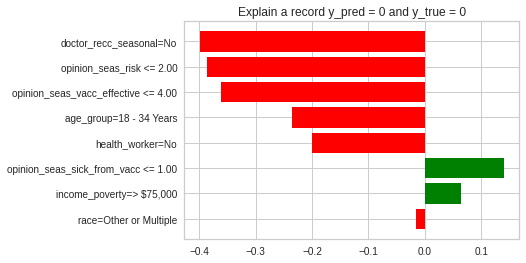
\includegraphics[width=0.6\linewidth]{images/Explanation_Lime_1.png}
    \caption{Lime explanation of a record with true target 0 and predicted target 0}
    \label{img:lime_1}
\end{figure}

In Figure \ref{img:lime_1} we show the result of a Lime Explanation, we considered the same instance we used with the local Shap explanation so that we can make a comparison.
You can see that features like the doctor's recommendation and the opinion on the efficacy of the vaccine effectiveness are important for the final prediction.


\textbf{Lore}

The last method we used for the local interpretability is Lore that gave us a set of rules. We explained the same instances also with Lore \cite{guidotti2018local} that gave us a set of rules and a set of counterfactuals that could lead the model to a different classification.
In the following list, we report the rules and the counterfactual of the record with prediction 0 and true value 0 that we also used in the previous local explanations.

\begin{itemize}
    \item Rule: $doctor\_recc\_seasonal <= 0.29$
    \item Rule: $opinion\_seas\_risk <= 2.50$
    \item Counterfactual: $opinion\_seas\_risk > 2.50$
    \item Counterfactual: $health\_worker > 0.50$
\end{itemize}


\subsection{Analysis of similar instances with different predictions}

To sum up the previous subsections and to prove how a different feature may affect the final prediction of the model we considered an instance of the seasonal dataset and we computed the cosine similarity with all the others instances of the dataset. We selected the most similar instances with the same target ("Vaccine") and a different prediction of the model ("No vaccine").
In Figure \ref{img:comparison_different_prediction_1} we show the Lime interpretation of instance predicted correctly and in \ref{img:comparison_different_prediction_1} the instance predicted incorrectly. We can note that the features $"opinion\_seas\_risk \ <= \ 2"$, $"opinion\_seas\_vacc\_effective \ <= \ 4"$ and $"age\_group=18-34"$ led the model to an incorrect prediction.


\begin{figure}
    \begin{minipage}{0.48\textwidth}
        \centering
        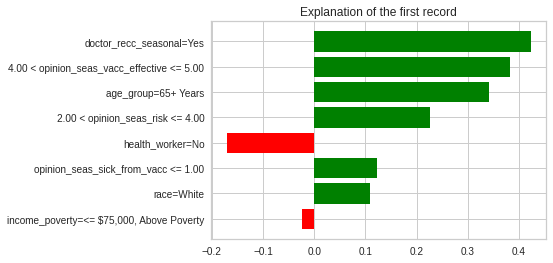
\includegraphics[width=\linewidth]{images/comparison_1.png}
        \caption{Instance with correct prediction}
        \label{img:comparison_different_prediction_1}
    \end{minipage}\hfill
    \begin{minipage}{0.48\textwidth}
        \centering
        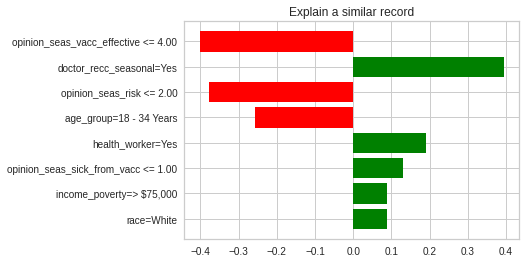
\includegraphics[width=\linewidth]{images/comparison_2.png}
        \caption{Similar instance with different prediction}
        \label{img:comparison_different_prediction_2}
    \end{minipage}
\end{figure}


\subsection{Global Explanation}

\subsubsection{Skater}

For the global explanation we used the Skater package, in particular, the updated version dates back to 2018 with some minor corrections by users \cite{skater}.
We cover the Global explanation of the models “Decision Tree” and “Random Forest” for H1N1 vaccine and “Decision Tree” and “XGBoost” for the “Seasonal Vaccine”.
For each dataset, we will apply the same global interpretation techniques.
The explanations we will be covering in this section are the following:

\begin{itemize}
    \item Feature Importance;
    \item Partial Dependence Plots (with one and two variables);
    \item Building Interpretable Models with Surrogate Tree-based Models (with images and text).
\end{itemize}

\textbf{Feature Importance}

We show in Figure \ref{img:skater1} the feature importance.

\begin{figure}[H]
    \centering
    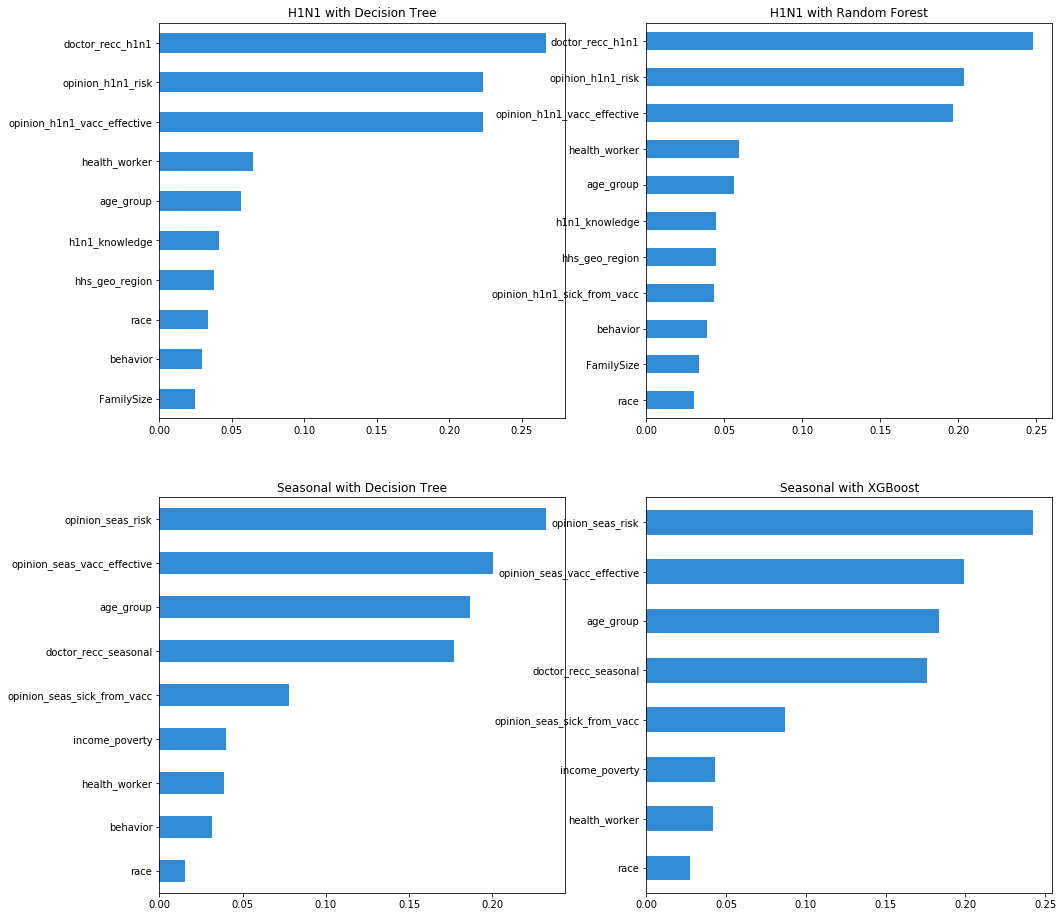
\includegraphics[width=\linewidth]{images/skater_1.png}
    \caption{}
    \label{img:skater1}
\end{figure}

For the H1N1 vaccine the most important features are (in descending order of importance):

\begin{itemize}
    \item $doctor\_rec\_h1n1$
    \item $opinion\_h1n1\_risk$
    \item $opinion\_h1n1\_effective$
\end{itemize}

For the seasonal vaccine are:

\begin{itemize}
    \item $opinion\_seas\_risk$
    \item $opinion\_seas\_vacc\_effective$
    \item $age\_grop$
\end{itemize}

This indicates that the opinion of the respondent regarding the efficacy of the vaccine and the risk of contracting the disease without a vaccine are relevant features.
We can also state that for the H1N1 vaccine the doctor's recommendation is the most important feature and it is not the same for the seasonal vaccine.


\textbf{Partial Dependence Plots}

Partial Dependence describes the impact of a feature on model prediction, keeping constant the other features in it. We are looking to the reasons that led people to get the vaccine, they must be interpreted according to a degree of importance.
In both types of vaccine, there are some features that have an increasing trend almost directly proportional to the number of people who get vaccinated.
These are the following features:
\begin{itemize}
    \item Level of knowledge about H1N1 flu;
    \item Opinion of the good effects of the vaccines;
    \item Risk of contracting flu without vaccine;
    \item Increasing income;
    \item There is a net increase of people who get vaccinated from 65 years onwards;
    \item Black or Hispanic people are less vaccinated than white or other races;
    \item The doctor's recommendation to carry out the vaccine has a positive effect and is more decisive in the H1N1 vaccine;
    \item More Respondents worry about getting sick from taking the seasonal flu vaccine more they don’t get the vaccine;
    \item Vaccination appears to be sensitive to the Respondent's residence;
    \item People with strict preventative behaviors get the vaccine;
    \item In families of 5 people, there is a sharp decrease in vaccination
\end{itemize}


\begin{figure}[H]
    \centering
    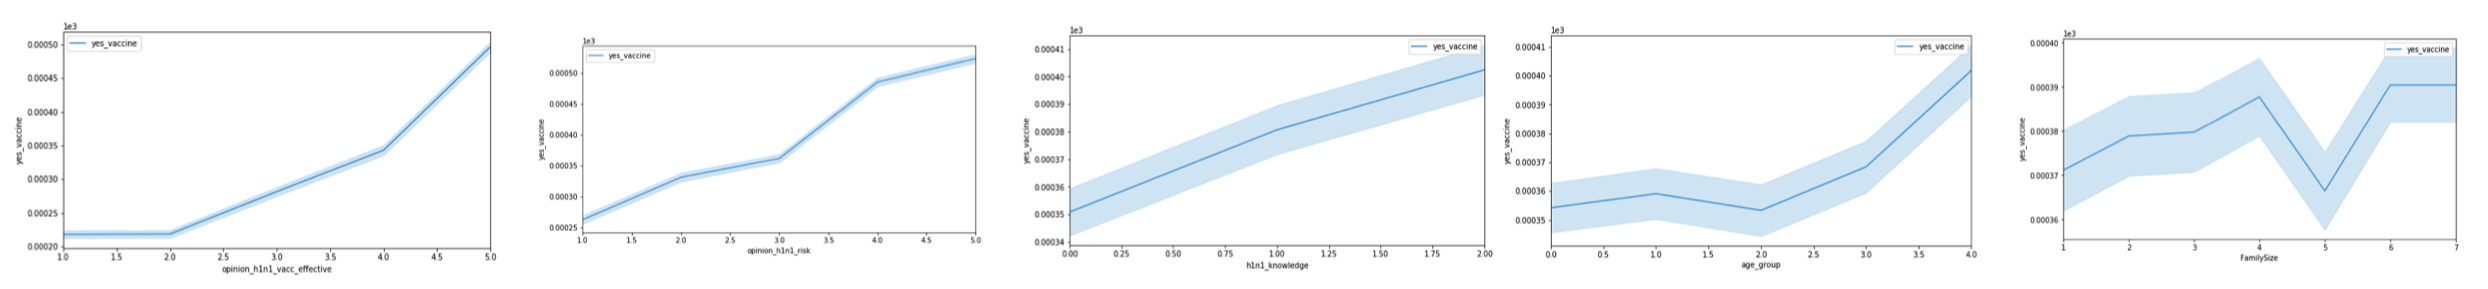
\includegraphics[width=\linewidth]{images/skater_2.png}
    \caption{}
    \label{skater2}
\end{figure}


\textbf{Building Interpretable Models with Surrogate Tree-based Models}

Now we will interpret the decision tree of H1N1 and seasonal vaccine. We considered only this interpretation due to the complexity of the tree branches.

\begin{itemize}
    \item With the H1N1 dataset, we can see the importance of the doctor's recommendation in encouraging patients to get the vaccine. 
    We notice this going up the tree from the leaf with the highest percentage $17.8\%$ of success for being classified with the class $yes\_vaccine$.
    Below this branch from root to leaf:

    $$(doctor\_rec\_h1n1 > 0.5)\ ->\ (opinion\_h1n1\_vacc\_effective \ > \ 3.5)\ ->$$
    $$(opinion\_h1n1\_risk > 1.5)\ ->\ (Family\_size\ <=\ 4.5)\ ->\ (H1N1\_knoledge \ >\ 0.5)$$

    The Associated explanation is:

    \begin{itemize}
        \item The doctor recommends the h1n1 vaccine
        \item The respondent's opinion on the efficacy of the h1n1 vaccine is “somewhat” or “very effective” 
        \item Respondent's opinion about the risk of getting sick with h1n1 flu without a vaccine is “somewhat low”, or “don’t know” or “somewhat high”, or “very high” 
        \item Family size $<=$ 4 
        \item Level of knowledge about H1N1 flu can be a “little or a lot of knowledge”.
    \end{itemize}

    \item With the Seasonal dataset, we can see from root to the leaf a strong rule ($class=yes\_vaccine$) with samples $15.7\%$.
    
    The Associated explanation is:
    \begin{itemize}
        \item Respondent's opinion about seasonal vaccine effectiveness is "very effective"
        \item The age group of respondents is $>=$ 45 years 
        \item Respondent's opinion about the risk of getting sick with seasonal flu without a vaccine can be “Don't know”, “Somewhat high” or “Very high”
        \item The respondent's race can be “White” or “other or multiple” 
        \item The respondent adopted all the good behaviours to prevent getting sick.
    \end{itemize}
\end{itemize}

\subsubsection{Shap}

Shap, from the Global point of view, gives us different tools: an interactive plot that shows different insights about the models, a summary plot to study the impact of each feature on the model's decisions, and a dependence plot that show the interaction between features in the model.
We plotted those charts for all our models. The interactive plot lets us understand for each feature which are the values that influence the labeling of unseen data as 0 or 1. Some features show behavior in line with expectations while other ones exhibit unexpected behavior for certain values. In particular, for all our models, both for seasonal flu and H1N1, it may be strange that $opinion\_seas\_vacc\_effective = 4$ imply the classification equal to 0 and that only $opinion\_seas\_sick\_from\_vacc = 1$ makes the classification tend towards 1.  In our dataset majority of respondents for whom $opinion\_seas\_vacc\_effective = 4$ are not vaccinated for the Seasonal flu and/or H1N1. This can be interpreted in two ways: our dataset is not quite representative for this feature or surprisingly in reality who believe that the vaccine is effective teds not to get the vaccine except for extreme cases ($opinion\_seas\_vacc\_effective = 5$). The same reasoning can be done for $opinion\_seas\_sick\_from\_vacc$.
We discovered also that the feature behavior is not discriminant for the classification, a good behavior does not imply that the respondent has done the vaccine and vice versa.
For H1N1 is strange that $opinion\_h1n1\_sick\_from\_vacc = 4$ makes the classification tend towards 1. This is probably due to the unbalance of the dataset that leads to a not discriminant interpretation of this feature with this value.

\begin{figure}[H]
    \centering
    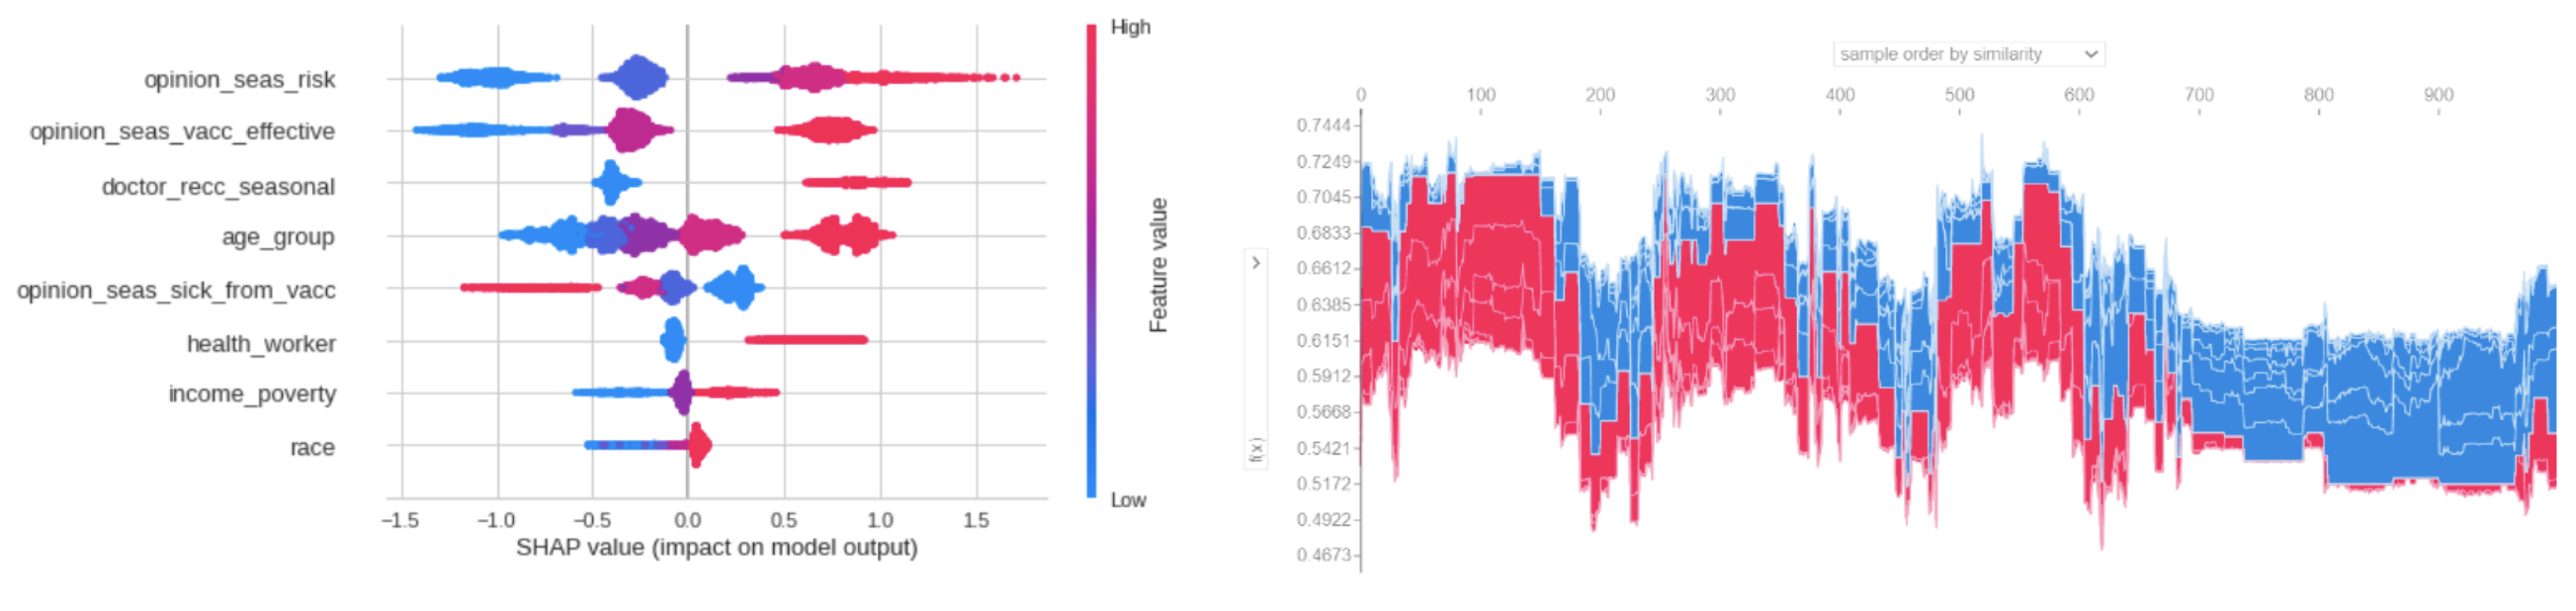
\includegraphics[width=\linewidth]{images/shap_global_1.png}
    \caption{Global explanation with Shap}
    \label{img:shap_global}
\end{figure}


\section{Use Cases}

At the end of our work, we analyzed the results of the explainers and in particular, we concentrated on the records that are classified as "No Vaccine" i.e. on the respondent that did not receive the seasonal and H1N1 vaccine.

Our goal was to understand why a certain respondent did not receive the vaccine and if their ideas and behavior could lead the model to this conclusion.
Regarding the classification, the respondents that did not receive the vaccine are the ones that have the following features:

\begin{itemize}
    \item They believe that the vaccine is not effective.
    \item They are young and they have no fear of taking the seasonal flu.
    \item Their doctor did not recommend the vaccine. This is an important feature to consider, especially for the H1N1 vaccine.
    \item Usually they are under the poverty line. This is an important point because the survey was made in the U.S.A. where health insurance is paid for.
    \item Usually they are Black or Hispanic or other minorities. We analyzed this feature of the model because it could be a racial bias of our model but in reality, we notice that this feature is always associated with the other features we have just described.
\end{itemize}

We guessed that considering these pieces of information we could use our research to make campaigns for the use of the vaccine directed to a certain type of population, for example, the young people that, especially during pandemics, could be a vector of influence.

Using the data collected during the H1N1 pandemic of 2009 it could also be possible to predict what part of the populations will most likely receive the Covid-19 vaccine and moreover it could be possible to activate targeted campaigns to raise awareness of the vaccine.




\section{Conclusion}

The first Milestone led us to know our dataset and to propose some possible changes that exploited during the Classification Phase.

The training set was divided into two data sets. One for the H1N1 flu and one for the seasonal, they have some common attributes while some attributes are typical for the type of the influence.
We believe that by dividing the dataset, it is possible to highlight the small differences between the two vaccines and create more suitable models for each.

We also found some similar datasets with surveys of the following years \cite{Next years} but they were too different from our dataset and we were not able to merge them.

The second Milestone allowed us to develop and test several different models giving us the opportunity to reason about them in terms of performances but also in terms of interpretability.
To develop these models we had to solve some troubles with the unbalanced dataset and also from this point of view we had the opportunity to test a lot of different balancing techniques.
Following the suggestions after the first midterm, we also studied in deep which of our features are more important and we demonstrated that our intuitions were good.

The third Milestone led us to an in-depth knowledge of the models we used during the previous Milestone. In particular, we were able to understand what features are more important for classification purposes.
Considering the importance of these features we were also able to understand whether our model had some bias or not.
During this Milestone, we also formulated some possible use cases of our project.


%
% ---- Bibliography ----
%
% BibTeX users should specify bibliography style 'splncs04'.
% References will then be sorted and formatted in the correct style.
%
% \bibliographystyle{splncs04}
% \bibliography{mybibliography}
%
\begin{thebibliography}{8}
    \bibitem{Dataset}
    U.S. Department of Health and Human Services (DHHS).
    National Center for Health Statistics. The National 2009
    H1N1 Flu Survey. Hyattsville, MD: Centers for Disease
    Control and Prevention, 2012. \url{https://www.cdc.gov/nchs/nis/data\_files\_h1n1.htm/}


    \bibitem{Driven Data}
    Flu Shot Learning: Predict H1N1 and Seasonal Flu Vaccines. \url{https://www.drivendata.org/competitions/66/flu-shot-learning/page/210/}

    \bibitem{Full Dataset}
    Datasets for the National 2009 H1N1 Flu Survey (NHFS) \url{ftp://ftp.cdc.gov/pub/Health\_Statistics/NCHS/Datasets/nis/nhfs/nhfspuf.dat}

    \bibitem{Next years}
    Surveys of the following years \url{https://www.cdc.gov/nchs/nis/data\_files.htm}

    \bibitem{GridSearchCV}
    GridSearchCV \url{https://scikit-learn.org/stable/modules/generated/sklearn.model_selection.GridSearchCV.html}

    \bibitem{RandomizedSearchCV}
    RandomizedSearchCV \url{https://scikit-learn.org/stable/modules/generated/sklearn.model_selection.RandomizedSearchCV.html}

    \bibitem{dtInterpretability}
    Interpretable Machine Learning - Decision Tree https://christophm.github.io/interpretable-ml-book/tree.html

    \bibitem{logisticInterpretability}
    Interpretable Machine Learning - Logistic Regression https://christophm.github.io/interpretable-ml-book/logistic.html

    \bibitem{molnar2019}
    Interpretable Machine Learning, Christoph Molnar, \url{https://christophm.github.io/interpretable-ml-book/} 2019, A Guide for Making Black Box Models Explainable.

    \bibitem{guidotti2018local}
    Local Rule-Based Explanations of Black Box Decision Systems, Riccardo Guidotti and Anna Monreale and Salvatore Ruggieri and Dino Pedreschi and Franco Turini and Fosca Giannotti, 2018

    \bibitem{lundberg2017unified}
    A Unified Approach to Interpreting Model Predictions, Scott Lundberg and Su-In Lee, 2017

    \bibitem{skater}
    Skater Github: https://github.com/oracle/Skater/tree/master/skater/core





\end{thebibliography}
\end{document}
}